% !TEX encoding = UTF-8
% !TEX TS-program = pdflatex
% !TEX root = ../tesi.tex
% !TEX spellcheck = it-IT

%**************************************************************
\chapter{Realizzazione}
\label{cap:realizzazione}
%**************************************************************

Questo capitolo contiene la descrizione delle attività svolte e dei problemi incontrati durate lo sviluppo dell'applicazione, la quale è stata sviluppata a partire dal prototipo precedentemente realizzato per valutare React Native.

L'attività di codifica è stata quindi organizzata in modo che venissero implementati di volta in volta dei determinati componenti, per soddisfare determinati requisiti, ottenendo così delle versioni intermedie e funzionanti dell'applicazione che sono state usate per effettuare delle demo all'interno dell'azienda.
\todo{da rivedere}

\section{Dal prototipo alla gallery}

Prima di iniziare lo sviluppo di nuove funzionalità sul prototipo è stato prima necessario adattarlo all'architettura progettata, modificano alcuni componenti.

La versione del prototipo che è stata utilizzata implementava già il pattern Flux mediante il modulo npm \texttt{flux}, ed era organizzata con due \textit{stores}, uno che teneva gestiva le immagini e uno che si occupava di gestire le fonti disponibili per le immagini.

Come prima cosa sono stati modificati gli \textit{stores} e le relative \textit{actions} secondo quando progettato, trasformando lo \textit{store} delle immagini in quello degli assets e lo \textit{store} delle fonti in quello dei nodi figli.

Inoltre, l'oggetto del prototipo che si occupava del recuperare i dati è stato modificato in modo che interroghi le API di WARDA e che gestisca l'autenticazione.

L'implementazione dell'autenticazione è stata semplice in quanto è bastata una variabile booleana per specificare se l'autenticazione era già stata effettuata e, nel caso non lo fosse, veniva prima richiesta e poi veniva effettuata la chiamata alle API vera e propria.

Non è stato necessario gestire cookie o quant'altro dal momento che l'oggetto \texttt{fetch} offerto da React Native per effettuare chiamate HTTP funziona come proxy del componente nativo di iOS che si occupa di gestire il traffico di rete e questo componente nativo gestisce in modo automatico i cookies.

Per quanto riguarda l'interfaccia grafica è stato necessario modificare la griglia in modo che visualizzare oggetti di tipo \texttt{Asset} e che implementasse lo scroll infinito.

Per implementare lo scroll infinito, il componente \texttt{ListView} di React Native, che sta alla base della visualizzazione a griglia, rende disponibile l'evento \texttt{onEndReached}, che viene sollevato ogni volta che l'utente raggiunge la fine della lista.

Tuttavia questa implementazione aveva due problemi:
\begin{itemize}
\item il caricamento dei nuovi dati iniziava quanto l'utente arrivava alla fine delle lista, quando poteva essere anticipato, in modo da migliorare ulteriormente l'esperienza d'uso;
\item in alcuni casi l'evento veniva sollevato troppe volte il che portava a caricare più volte lo stesso blocco di dati.
\end{itemize}

Questi problemi sono stati risolti implementano lo scroll infinito utilizzando l'evento \texttt{onScroll} della \texttt{ListView}, che viene sollevato ogni volta che l'utente esegue uno scroll.

Alla funzione che gestisce l'evento viene passato come parametro un oggetto con tutte le informazioni relative all'evento, in questo modo è stato possibile richiedere il caricamento di ulteriori dati ad una distanza personalizzabile dalla fine ed effettuare maggiori controlli in modo da evitare che la stessa porzione di dati venisse caricata più volte.

\begin{lstlisting}[language=JavaScript, caption=Funzione che gestisce l'evento onScroll della griglia che visualizza gli assets]
function onScroll(args) {
  var scrollY = args.nativeEvent.contentOffset.y;
  var height = args.nativeEvent.contentSize.height;
  var visibleHeight = args.nativeEvent.layoutMeasurement.height;

  if (scrollY > height - 2 * visibleHeight){
    //Se mancano menod di due schermate alla fine della lista, richiedo il caricamento di ulteriori dati
    //Per evitare che il caricamento venga effettuato troppe volte controllo che i dati siano cambiati rispetto all'ultima volta che ho effettuato il caricamento.
    if (_dataChanged){ //Viene settata a true quando il componente riceve dei dati nuovi
      _dataChanged = false;
      var downloadStarted = this.props.onLoadMoreData();
      var temp = this.props.assets.concat([{loading:true}]); //Visualizza un'indicatore di caricamento
      this.setState({
        downloading: downloadStarted,
        dataSource: dataSource.cloneWithRows(temp)
      });
    }
  }
}
\end{lstlisting}

Al termine di questa prima fase l'applicazione è in grado di visualizzare il contenuto di un nodo e di visualizzare la lista dei nodi disponibili, anche se non è ancora possibile navigare tra i vari nodi.

\section{Sistema di navigazione}

Successivamente è stato sviluppato il sistema di navigazione completo, il quale fornisce la possibilità all'utente di scendere o risalire lungo la gerarchia dei nodi.

La maggior parte delle modifiche effettuate in questa fase riguardano \texttt{NodesStores} in quanto è stato necessario implementare un sistema che tenga traccia del percorso effettuato dall'utente lungo la gerarchia della gallery.

Questo sistema è inoltre vincolato dal funzionamento delle API di WARDA, le quali, dato l'id di un nodo, permettono solamente di ottenere le informazioni riguardanti i nodi figli o gli assets in esso contenuti.

\`E stato quindi necessario implementare un sistema che, quando viene richiesto il caricamento dei nodi a partire da un determinato URL, sia in grado di recuperare un oggetto \texttt{Node} contenente le informazioni relative al nodo padre dei nodi di cui è richiesto il caricamento.
Inoltre, questo sistema deve essere in grado di tenere traccia del percorso che l'utente ha effettuato durante la navigazione della gallery.

Per far funzionare il tutto è stato necessario modificare la funzione che carica i nodi all'interno dello \textit{store} in modo che, prima di caricare i nuovi nodi, cerchi tra gli oggetti \texttt{Node} presenti all'interno dello \textit{store} l'oggetto rappresentante il nodo padre dei nuovi nodi, utilizzano l'URL dal quale sono stati scaricati i nuovi dati.
L'oggetto viene poi inserito in coda ad un'array contenente tutti i nodi appartenenti al ramo della gallery che l'utente sta visualizzando.

Nel caso che l'utente stia tornando ad un nodo precedente, anziché effettuare l'inserimento dell'oggetto nodo, viene rimosso l'ultimo elemento dell'array. 

\begin{lstlisting}[language=JavaScript, caption=NodesStore - Caricamento dei nodi]
//_nodes --> Array con i nodi correntemente visualizzati
//_nodeHierarchy --> Array con i nodi visualizzati dall'utente, è inizializzato come array vuoto
function loadNodes(parentUrl, nodes) {

  if (_nodesHierarchy.length === 0){
    //E' il primo caricamento dei dati, la gerarchia dei nodi inizia da un nodo "finto" che funziona da radice
    //in quanto le API di WARDA non forniscono informazioni riguardanti il nodo radice di una gallery
    _nodesHierarchy.push({isRoot:true,text:'', urlContentDataStore:'', urlChildrenStore:''});
  } else {
    //Ultimo nodo del ramo della gerarchia dei nodi che l'utente ha visualizzato
    var lastNode = _nodesHierarchy[_nodesHierarchy.length -1];

    if (lastNode.urlChildrenStore.length < parentUrl.length){
     //Se l'url dell'ultimo nodo è più corto (più alto in gerarchia) dell'url del nodo corrente, vuol dire che l'utente sta scendendo lungo il ramo
      //Il nodo corrente (quello di cui sto caricando i figli) è il nodo che ha urlContentDataStore == parentUrl e che si trova correntemente in memoria
      var currentNode = _nodes.filter((item) => item.urlChildrenStore === parentUrl)[0];
     //Aggiungo il nodo corrente in coda
      _nodesHierarchy.push(currentNode);
    } else {
      //L'url dell'ultimo nodo è più lungo dell'url del nodo corrente, vuol dire che sto risalendo lungo il ramo
      //Faccio un pop per togliere l'ultimo elemento dell'array
      _nodesHierarchy.pop();
    }
  }
  //Aggiornamento dei nodi
  _nodes = nodes;
}
\end{lstlisting}


\section{Sistema dei filtri}

Nonostante la struttura del sistema dei filtri applicabili ai contenuti di una gallery risulti complesso, le API di WARDA forniscono un livello di astrazione tale da rendere l'implementazione lato client semplice.

Infatti, per inserire il sistema di filtri all'interno dell'applicazione è bastato implementare \texttt{FiltersStore} per tenere traccia dei filtri applicati ed modificare alcuni metodi di \texttt{AssetsActions} e di \texttt{WardaFetcher} in modo che prendessero un ulteriore parametro con i filtri da applicare.

\begin{lstlisting}[language=JavaScript, caption=WardaFetcher - Caricamento degli assets considerando i filtri]
function fetchContents(contentUrl,start, filters){
  var filtersString = '';
  if (!contentUrl){ contentUrl = '';}
  if (!start){start = 0;}

  if (filters && filters.length > 0){
    filtersString = JSON.stringify(filters);
    filtersString = '&filter='+encodeURIComponent(filtersString);
  }
  var url=`${WARDA_URL+contentUrl}?start=${start}&limit=${Config.PAGE_SIZE}${filtersString}`;

  return authenticatedFetch(url)
    .then((response) => response.json());
}
\end{lstlisting}

Per quanto riguarda l'implementazione grafica è stato utilizzato il componente \texttt{react-native-popover}\footnote{\url{https://github.com/jeanregisser/react-native-popover}} presente in npm, il quale permette di visualizzare un popover contenente altri componenti di React Native e che in questo caso è stato utilizzato per visualizzare la lista dei filtri.

\section{Visualizzazione di dettaglio}

Durante questa fase è stato implementato il componente \texttt{AssetDetailPage} che viene visualizzato quanto l'utente effettua un tap sull'immagine di asset nella visualizzazione a griglia. 

Una caratteristica di questa pagina è che quando l'utente esegue uno swipe sull'immagine dell'asset, devono essere visualizzati i dettagli dell'asset precedente o successivo rin base alla direzione dello swipe, ottenendo così una visualizzazione della gallery a carosello.

L'ordine di visualizzazione degli assets nel carosello deve seguire l'ordine della griglia di \texttt{GalleryPage}, inoltre, dal momento che la visualizzazione a griglia può contenere solamente alcuni degli assets disponibili, è necessario che anche dalla visualizzazione a carosello sia possibile effettuare il download di ulteriori assets.

Nell'implementare questo sistema si sono visti i alcuni dei vantaggi dell'architettura Flux, in quanto è bastato aggiungere due metodi a \texttt{NodesStore} per permette di recuperare l'asset precedente o successivo di un determinato oggetto \texttt{Asset} e di fornire a \texttt{AssetDetailPage} i dati che sono presenti su \texttt{NodesStore}.

Per la gestione del caricamento di ulteriori assets viene utilizzata la stessa \textit{action} che utilizza \texttt{GalleryPage} e, dal momento che i dati presenti in \texttt{NodesStore} sono comuni ad entrambe le pagine, quando \texttt{AssetDetailPage} richiede il caricamento di ulteriori dati, questi diventano subito disponibili anche per \texttt{GalleryPage} e viceversa, riducendo così il numero di download necessari.

Una volta ultimato il carosello è stato implemento il componente \texttt{NetworkImage} in modo che l'utente ricevesse un feedback riguardo il caricamento dell'immagine.
Questo si è reso necessario dal momento che l'immagine visualizzata in questa pagina è ad elevata risoluzione e il più delle volte il download richiede una quantità di tempo significativa.

L'implementazione di questo componente ha sofferto per un po' di tempo di alcuni problemi che derivavano da un bug del componente \texttt{Image} di React Native.
La versione \texttt{0.9.0-rc} del framework ha poi risolto questi bug, rendendo così possibile l'implementazione finale di \texttt{NetworkImage}.


\section{Animazioni}

Una volta soddisfatti i requisiti obbligatori e desiderabili si è passati all'introduzione di alcune animazioni, sfruttando le API offerte da React Native, che hanno permesso di ottenere animazioni fluide con delle prestazioni paragonabili a quelle delle animazioni native.

Le prime animazioni introdotte riguardano la comparsa e la scomparsa della lista dei nodi nella visualizzazione della gallery e della lista dei dettagli di un asset nella visualizzazione di dettaglio.

Queste animazioni sono state ottenute utilizzando le API \texttt{LayoutAnimation} che permettono di renderizzare l'interfaccia grafica in modo che le modifiche risultino animate.

\begin{lstlisting}[language=JavaScript, caption=AssetDetailPage - Animazione della comparsa/scomparsa lista dei dettagli]
function onDetailButtonPress() {
  LayoutAnimation.easeInEaseOut(); //Imposta l'animazione
  this.setState({detailsVisible: !this.state.detailsVisible}); //Modifica lo stato del componente causandone il re-rendering
}
\end{lstlisting}

Come si può notare dall'esempio sopra riportato l'implementazione di queste animazioni risulta estremamente semplice.

Una volta inserite tutte le animazioni necessarie alla modifica del layout si è animato lo swipe della visualizzazione a carosello di \texttt{AssetDetailPage}.

Questa animazione ha richiesto l'utilizzo delle API \texttt{Animated} che permettono di definire animazioni più complesse.

Per funzionare, queste API utilizzano dei particolari componenti grafici, il cui stile dipende da determinati valori che possono essere modificati in vario modo. La modifica di questi valori comporta quindi la modifica dello stile del componente in modo animato.

Ad esempio, il seguente codice implementa l'animazione dell'immagine in modo che l'immagine segua lo swipe dell'utente.

\begin{lstlisting}[language=JavaScript, caption=AssetDetailImage - Spostamento dell'immagine allo swipe delll'utente]
//costruttore di AssetDetailPage

this.state.panX = new Animated.Value(0); //Variabile che rappresenta lo spostamento dell'immagine
this.state.swipePanResponder = PanResponder.create({ //Oggetto che si occupa di rilevare le gesture dell'utente
  ...
  onPanResponderMove: Animated.event([null, {dx: this.state.panX}]), //All'evento onPanResponderMove, che viene sollevato quando l'utente esegue un pan (equivalente del drag'n'drop nei dispositivi touchscreen) viene collegata la variabile panX, in modo che il valore della variabile venga modificato e che la modifica venga effettuata in modo animato
  ...
});

//funzione di rendering dell'immagine
return (
  <Animated.View
    {...this.state.swipePanResponder.panHandlers} //Il gestore degli eventi viene collegato alla View
    style={..., {
      transform: [{translateX: this.state.panX},  ], //Il valore dello spostamento viene associato allo stile della View, in particolare alla traslazione sull'asse X
    }]}>
    	//Codice che visualizza l'immagine
  </Animated.View>
);
\end{lstlisting}

L'effetto prodotto dal quel codice è il seguente:

\vspace{1em}
\noindent
\begin{minipage}{\textwidth}
  \begin{minipage}[b]{0.49\textwidth}
    \centering
    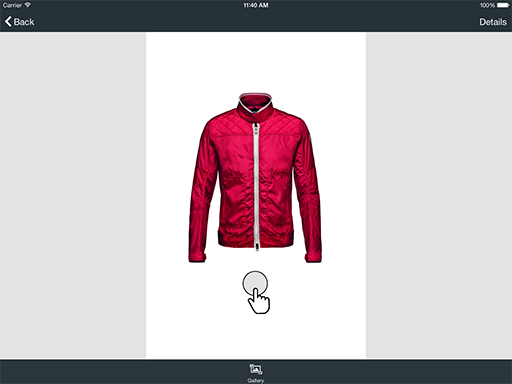
\includegraphics[scale=0.25]{../immagini/swipe-start}
      \captionof{figure}{Immagine all'inzio dello swipe}
	\end{minipage}
	  \hfill
  \begin{minipage}[b]{0.49\textwidth}
    \centering
  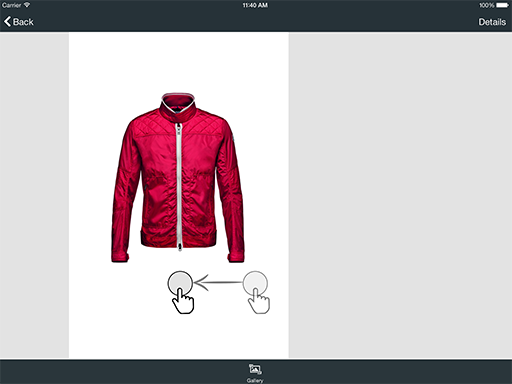
\includegraphics[scale=0.25]{../immagini/swipe-follow}
      \captionof{figure}{Immagine durante lo swipe}
  \end{minipage}
\end{minipage}

\vspace{1em}
Tuttavia, il codice sopra riportato sposta l'immagine in base al pan effettuato dall'utente e non esegue nessuna animazione quando lo swipe viene completato e viene visualizzata un'altra immagine.

Infatti, nelle applicazioni native, una volta che l'utente ha completato uno swipe, l'immagine corrente viene mandata ``\textit{fuori dallo schermo}'' in modo animato, per poi visualizzare la nuova immagine.

Mentre se l'utente non completa lo swipe, l'immagine viene fatta ritornare alla posizione iniziale, sempre in modo animato.

Per implementare ciò, è stato necessario modificare il gestore dello swipe, in modo che esegua le animazioni dell'immagine quando l'utente completa o annulla lo swipe.

Il codice utilizzato per effettuare le altre animazioni è il seguente:
\begin{lstlisting}[language=JavaScript, caption=AssetDetailPage - Animazione dello swipe]
this.state.swipePanResponder = PanResponder.create({
  ...
  onPanResponderRelease: (e, gestureState) => { //Funzione che viene invocata quando l'utente termina la gesture
    var swipeSize = 150; //Dimensione dello swipe in pixel
    
    //gestureState.dx rappresenta lo spostamento sull'asse X effettuato dall'utente
    if (Math.abs(gestureState.dx)>swipeSize){
      //L'utente ha completato lo swipe
      var toValue;
      
      if (gestureState.dx > 0) {
        toValue = 1000; //Valore in modo che l'immagine venga renderizzata offscreen
      } else {
        toValue = -1000;
      }
     
      //Mando l'immagine offscreen in modo animato, la direzione dipende dalla direzione della gesture (segno di gestureState.dx)
      Animated.spring(this.state.panX, {
        toValue,
        velocity: gestureState.vx,
        tension: 10,
        friction: 3,
      }).start(); //Avvio dell'animazione
      
      this.state.panX.removeAllListeners();
      var id = this.state.panX.addListener(function({value}){ 
      	//Aggiungo un listener all'esecuzione dell'animazione in modo di riuscire a capire quando l'immagine è finita fuori dallo schermo
        if (Math.abs(value) > 400) { //L'immagine è fuori dallo schermo
          this.state.panX.removeListener(id);
          
          var loading = (value > 0)? this.showPreviousAsset() : this.showNextAsset();
          if (loading){
            //C'è una nuova immagine da visualizzare
            this.state.panX.setValue(-toValue); //Posiziona l'immagine dalla parte opposta dello schermo
            Animated.spring(this.state.panX, { //Animazione che fa "entrare" la nuova immagine dalla parte opposta dello schermo
              toValue:0,
              velocity: gestureState.vx,
              tension:1,
              friction:6,
            }).start();
          } else {
          	//Non c'è nessun immagine da visualizzare, viene effettuata l'animazione che riporta l'immagine alla posizione iniziale
            Animated.spring(this.state.panX, {
              toValue:0,
              velocity: gestureState.vx,
              tension:1,
              friction: 4
            }).start();
          }
        }
      }.bind(this));
    } else {
      //L'utente non ha completato lo swipe, l'immagine deve tornare alla posizione iniziale in modo animato
      Animated.spring(this.state.panX, {
        toValue:0,
        velocity: gestureState.vx,
       }).start();
    }
  }
});
\end{lstlisting}

Sfruttando le stesse API si è inoltre provato da implementare il pinch-to-zoom, per permettere all'utente di zoomare l'immagine.

Tuttavia il pinch-to-zoom è una gesture complessa che combina più gesture:
\begin{itemize}
\item pinch, per regolare lo zoom;
\item pan, per spostare l'immagine una volta zoomata;
\item swipe, per cambiare l'immagine.
\end{itemize}

\`E stata effettuata un'implementazione parziale di questa gesture che è risultata poco performante e pertanto si è deciso, in accordo con il tutor aziendale, di non proseguire lo sviluppo di tale funzionalità.

\section{Gestione degli errori}

Nell'ultima fase si è stata implementata la gestione degli errori di connessione.

Le versioni precedenti dell'applicazione, infatti, non gestivano gli errori di comunicazione con il server, e nel caso se ne verificasse uno, i vari indicatori di attività rimanevano attivi fino al riavvio dell'applicazione.

\`E stato quindi implementato \texttt{ErrorsStore} in modo che fosse possibile memorizzare i vari messaggi d'errore, inoltre, sono state modificati tutti i metodi che creano delle azioni, in modo che se la promessa ritornata dai metodi di \texttt{WardaFetcher} fallisce, anziché eseguire il \textit{dispatch} normale dell'azione, richiedano ad \texttt{ErrorsActions} la creazione di un errore di rete, mediante il metodo \texttt{networkError(errorData)}.

La visualizzazione dei messaggi d'errore è stata affidata al componente di navigazione principale dell'applicazione, in modo quando si verifichi un errore venga renderizzato il messaggio al posto della tabbar.

\`E stato inoltre modificato il componente \texttt{NetworkImage} in modo che nel caso si verifichi un errore durante il caricamento dell'immagine venga visualizzato un messaggio d'errore al posto di un'immagine grigia.
